\documentclass[11pt]{article}
\usepackage{calc}
\usepackage[margin={1in,0.5in},footskip=0in]{geometry}
\usepackage[miniquiz]{hwk}
\usepackage{tikz, pgfplots}

\renewcommand{\theclass}{math 1300}
\renewcommand{\dateinfo}{October 2, 2012}
\renewcommand{\theassignment}{Quiz 4}

\begin{document}
\pagestyle{empty}
\newsavebox{\quizfront}
\begin{lrbox}{\quizfront}
\begin{minipage}[top][4.5in][t]{\textwidth} \setlength{\parindent}{1.5em}
\drawtitle
\vspace{-0.5in}
\begin{enumerate}

\item On the axes below, graph a function $g(x)$ such that:
  \begin{itemize}
  \item $g''(x)$ is always positive,
  \item $g'(x) \geq 0$ when $x \geq 2$,
  \item $g'(x) \leq 0$ when $x < 2$.
  \end{itemize}
  
  \begin{center}
    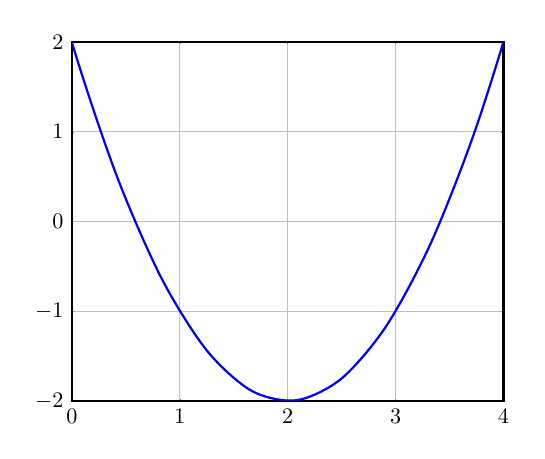
\begin{tikzpicture}[scale=0.8]
      \begin{axis}[ 
	xlabel={},
	ylabel={},
	xmin=0,
	xmax=4,
	ymin=-2,
	ymax=2,
	xtick={0,1,2,3,4},
	ytick={-2,-1,0,1,2},
	major tick length={1},
	grid=major,
	line width=1pt,]
        \addplot [smooth, blue] {(x-2)^2-2}; 

      \end{axis}
    \end{tikzpicture}
  \end{center}

\end{enumerate}

\hfill\textsc{over} $\longrightarrow$


\end{minipage}
\end{lrbox}

%%%%%%%%%%%%%%%%%%%%%%%%%%%%%%%%%%%%%%%%%%%%%%%%%%%%%%
%%%% This is for the back of the quiz
%%%%%%%%%%%%%%%%%%%%%%%%%%%%%%%%%%%%%%%%%%%%%%%%%%%%%%
\newsavebox{\quizback}
\begin{lrbox}{\quizback}
\begin{minipage}[top][4.5in][t]{\textwidth} \setlength{\parindent}{1.5em}
\begin{enumerate}
\item[2.] Let $f(t)$ be the number of inches of snow that have fallen since
  midnight, where $t$ is the time in hours. Interpret the following in
  practical terms, giving units.
  \begin{enumerate}
  \item $f(7) = 8$
    \vfill
    {\color{blue}
      Eight inches of snow have fallen by 7\textsc{am}.
    }
    \vfill
  \item $f'(4) = 2$
    \vfill
    {\color{blue}
      Approximately two inches of snow will fall between 4\textsc{am}
      and 5\textsc{am}.
    }
    \vfill
  \end{enumerate}

\end{enumerate}
\end{minipage}
\end{lrbox}

%%%%%%%%%%%%%%%%%%%%%%%%%%%%%%%%%%%%%%%%%%%%%%%%%%%%%%
%%%%
%%%% Now we make two copies of the ``quizfront'' box
%%%%
%%%%%%%%%%%%%%%%%%%%%%%%%%%%%%%%%%%%%%%%%%%%%%%%%%%%%%%
\noindent \usebox{\quizfront}
\vfill
\noindent \usebox{\quizback}

%%%% Uncomment the rest to have a two-sided quiz.
%\pagebreak
%\noindent \usebox{\quizback}
%\vfill
%\noindent \usebox{\quizback}
\end{document}